\documentclass[a4paper]{article}

\usepackage{Sweave} %--------------------------------!
\usepackage{amsmath}
\usepackage{amssymb}
\usepackage{fancyhdr}
\usepackage[usenames, dvipsnames]{color}
\usepackage{verbatim}

\oddsidemargin0cm
\topmargin-2cm     %I recommend adding these three lines to increase the
\textwidth16.5cm   %amount of usable space on the page (and save trees)
\textheight23.5cm

\newcommand{\question}[2] {\vspace{.25in} \hrule\vspace{0.5em}
\noindent{\bf #1: #2} \vspace{0.5em}
\hrule \vspace{.10in}}
\renewcommand{\part}[1] {\vspace{.10in} {\bf (#1)}}

\newcommand{\myname}{Xuan Han}
\newcommand{\myhusky}{han.xua@husky.neu}
\newcommand{\myhwnum}{1}

\setlength{\parindent}{0pt}
\setlength{\parskip}{5pt plus 1pt}

\pagestyle{fancyplain}
\lhead{\fancyplain{}{\textbf{HW\myhwnum}}}      % Note the different brackets!
\rhead{\fancyplain{}{\myname\\ \myhusky}}
\chead{\fancyplain{}{8-9}}


\begin{document}
\Sconcordance{concordance:introduction.tex:introduction.Rnw:%
1 47 1 1 2 4 0 1 2 2 1 1 2 18 0 1 2 6 1 1 2 25 0 1 2 6 1 1 2 40 0 1 1 3 %
0 1 2 6 1 1 2 5 0 1 2 12 1 1 2 1 0 1 3 1 0 1 2 4 1 6 0 1 2 1 0 1 3 6 0 %
1 3 19 1 1 2 1 0 9 1 4 0 1 2 7 1 1 2 26 0 1 2 19 1 1 2 12 0 1 2 20 1 1 %
2 1 0 2 1 14 0 1 1 21 0 1 2 26 1 1 2 1 0 3 1 3 0 1 2 1 1 1 2 9 0 1 2 2 %
1 1 2 7 0 1 1 7 0 1 2 2 1 1 2 1 0 3 1 6 0 1 1 6 0 1 1 8 0 1 2 7 1 1 2 5 %
0 2 2 1 0 1 2 1 0 2 1 1 2 1 0 1 2 1 0 1 2 1 0 1 2 1 0 1 2 1 0 1 2 5 0 1 %
2 31 1}


\title{Data Mining Assignment \myhwnum}
\author{\myname \\
        \myhusky}
\date{\today}
\maketitle

\medskip
\thispagestyle{plain}

\question{8}{College data set explore}
Explore:
\begin{enumerate}
\item Instead of loading csv file from disk, I Installed the dateset from ISLR
\begin{Schunk}
\begin{Sinput}
> library(ISLR)
\end{Sinput}
\end{Schunk}


\item Look into College data set by using head
\begin{Schunk}
\begin{Sinput}
> head(College, 2)
\end{Sinput}
\begin{Soutput}
                             Private Apps Accept Enroll Top10perc Top25perc
Abilene Christian University     Yes 1660   1232    721        23        52
Adelphi University               Yes 2186   1924    512        16        29
                             F.Undergrad P.Undergrad Outstate Room.Board Books
Abilene Christian University        2885         537     7440       3300   450
Adelphi University                  2683        1227    12280       6450   750
                             Personal PhD Terminal S.F.Ratio perc.alumni Expend
Abilene Christian University     2200  70       78      18.1          12   7041
Adelphi University               1500  29       30      12.2          16  10527
                             Grad.Rate
Abilene Christian University        60
Adelphi University                  56
\end{Soutput}
\end{Schunk}
{
\colorbox{BurntOrange}{\textbf{discovery1:}}\color{red}\\
Each row stand for a university and columns represent feature or properties of the university
}


\item Another good way to inspect our data by using str() fucntion
\begin{Schunk}
\begin{Sinput}
> str(College)
\end{Sinput}
\begin{Soutput}
'data.frame':	777 obs. of  18 variables:
 $ Private    : Factor w/ 2 levels "No","Yes": 2 2 2 2 2 2 2 2 2 2 ...
 $ Apps       : num  1660 2186 1428 417 193 ...
 $ Accept     : num  1232 1924 1097 349 146 ...
 $ Enroll     : num  721 512 336 137 55 158 103 489 227 172 ...
 $ Top10perc  : num  23 16 22 60 16 38 17 37 30 21 ...
 $ Top25perc  : num  52 29 50 89 44 62 45 68 63 44 ...
 $ F.Undergrad: num  2885 2683 1036 510 249 ...
 $ P.Undergrad: num  537 1227 99 63 869 ...
 $ Outstate   : num  7440 12280 11250 12960 7560 ...
 $ Room.Board : num  3300 6450 3750 5450 4120 ...
 $ Books      : num  450 750 400 450 800 500 500 450 300 660 ...
 $ Personal   : num  2200 1500 1165 875 1500 ...
 $ PhD        : num  70 29 53 92 76 67 90 89 79 40 ...
 $ Terminal   : num  78 30 66 97 72 73 93 100 84 41 ...
 $ S.F.Ratio  : num  18.1 12.2 12.9 7.7 11.9 9.4 11.5 13.7 11.3 11.5 ...
 $ perc.alumni: num  12 16 30 37 2 11 26 37 23 15 ...
 $ Expend     : num  7041 10527 8735 19016 10922 ...
 $ Grad.Rate  : num  60 56 54 59 15 55 63 73 80 52 ...
\end{Soutput}
\end{Schunk}
{
\colorbox{BurntOrange}{\textbf{discovery2:}}\color{red}\\
Here we find that there are 777 universities and there are 18 features for each university
}


\item Use summary() function to produce a numerical summary of the variables in the data set
\begin{Schunk}
\begin{Sinput}
> summary(College)
\end{Sinput}
\begin{Soutput}
 Private        Apps           Accept          Enroll       Top10perc    
 No :212   Min.   :   81   Min.   :   72   Min.   :  35   Min.   : 1.00  
 Yes:565   1st Qu.:  776   1st Qu.:  604   1st Qu.: 242   1st Qu.:15.00  
           Median : 1558   Median : 1110   Median : 434   Median :23.00  
           Mean   : 3002   Mean   : 2019   Mean   : 780   Mean   :27.56  
           3rd Qu.: 3624   3rd Qu.: 2424   3rd Qu.: 902   3rd Qu.:35.00  
           Max.   :48094   Max.   :26330   Max.   :6392   Max.   :96.00  
   Top25perc      F.Undergrad     P.Undergrad         Outstate    
 Min.   :  9.0   Min.   :  139   Min.   :    1.0   Min.   : 2340  
 1st Qu.: 41.0   1st Qu.:  992   1st Qu.:   95.0   1st Qu.: 7320  
 Median : 54.0   Median : 1707   Median :  353.0   Median : 9990  
 Mean   : 55.8   Mean   : 3700   Mean   :  855.3   Mean   :10441  
 3rd Qu.: 69.0   3rd Qu.: 4005   3rd Qu.:  967.0   3rd Qu.:12925  
 Max.   :100.0   Max.   :31643   Max.   :21836.0   Max.   :21700  
   Room.Board       Books           Personal         PhD        
 Min.   :1780   Min.   :  96.0   Min.   : 250   Min.   :  8.00  
 1st Qu.:3597   1st Qu.: 470.0   1st Qu.: 850   1st Qu.: 62.00  
 Median :4200   Median : 500.0   Median :1200   Median : 75.00  
 Mean   :4358   Mean   : 549.4   Mean   :1341   Mean   : 72.66  
 3rd Qu.:5050   3rd Qu.: 600.0   3rd Qu.:1700   3rd Qu.: 85.00  
 Max.   :8124   Max.   :2340.0   Max.   :6800   Max.   :103.00  
    Terminal       S.F.Ratio      perc.alumni        Expend     
 Min.   : 24.0   Min.   : 2.50   Min.   : 0.00   Min.   : 3186  
 1st Qu.: 71.0   1st Qu.:11.50   1st Qu.:13.00   1st Qu.: 6751  
 Median : 82.0   Median :13.60   Median :21.00   Median : 8377  
 Mean   : 79.7   Mean   :14.09   Mean   :22.74   Mean   : 9660  
 3rd Qu.: 92.0   3rd Qu.:16.50   3rd Qu.:31.00   3rd Qu.:10830  
 Max.   :100.0   Max.   :39.80   Max.   :64.00   Max.   :56233  
   Grad.Rate     
 Min.   : 10.00  
 1st Qu.: 53.00  
 Median : 65.00  
 Mean   : 65.46  
 3rd Qu.: 78.00  
 Max.   :118.00  
\end{Soutput}
\begin{Sinput}
> attach(College)
\end{Sinput}
\end{Schunk}
{
\colorbox{BurntOrange}{\textbf{discovery3:}} \color{red}\\
From this feature summary we can see that most of the universities are private which is about 72\% percent. Fulltime undergraduate students are much more than part-time undergraduate students. And so on
}


\item Use pairs() function to produce a scatterplot matrix of the first the columns
\begin{Schunk}
\begin{Sinput}
> pairs(College[, 1:10])
\end{Sinput}
\end{Schunk}
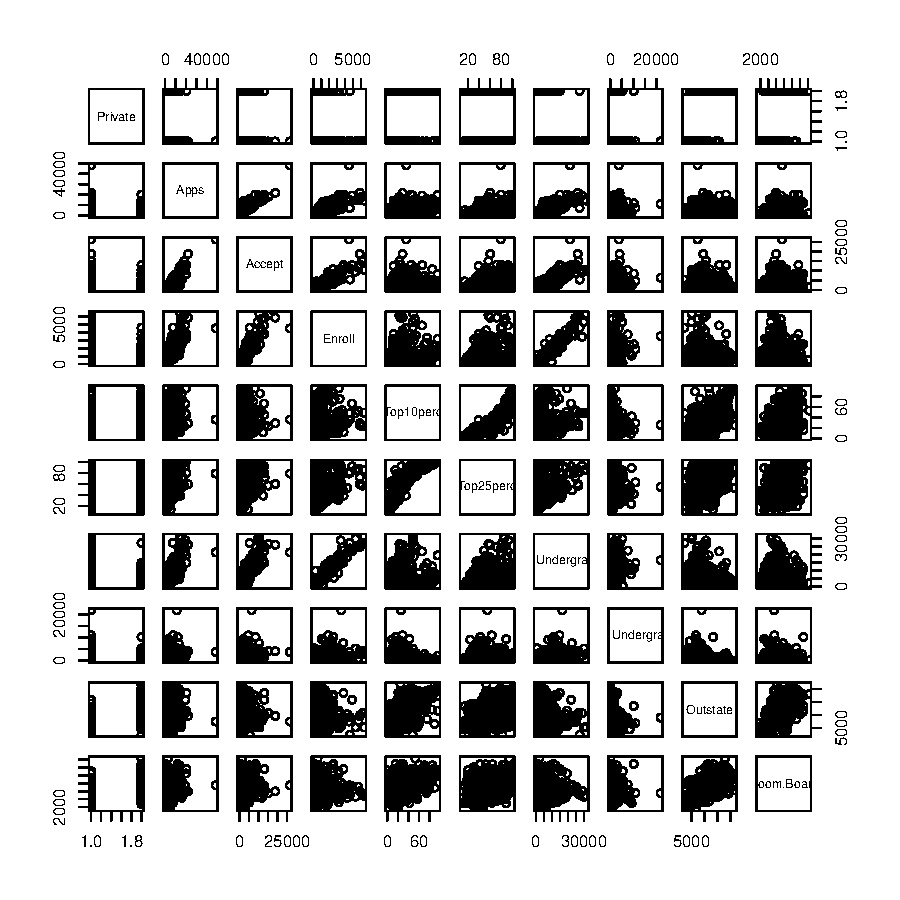
\includegraphics{introduction-pairs}

{
\colorbox{BurntOrange}{\textbf{discovery4:}}\color{red}\\
This command really gives us whole bunch of usefull information. For example: (1) we can see that private school have more top10\% students than public school; (2) application numbers and enroll numbers are basically linear relationship; (3) The more top10\% student, the more room and board costs; and so on.
}


\item Use the plot() function to produce side-by-side boxplots of \textit{Outstate} versus \textit{private}
\begin{Schunk}
\begin{Sinput}
> boxplot(Outstate ~ Private, College, ylab = "Outstate", xlab = "Private",
+         main = "Outstate vs. Private", col = rainbow(2), varwidth = T)
\end{Sinput}
\end{Schunk}
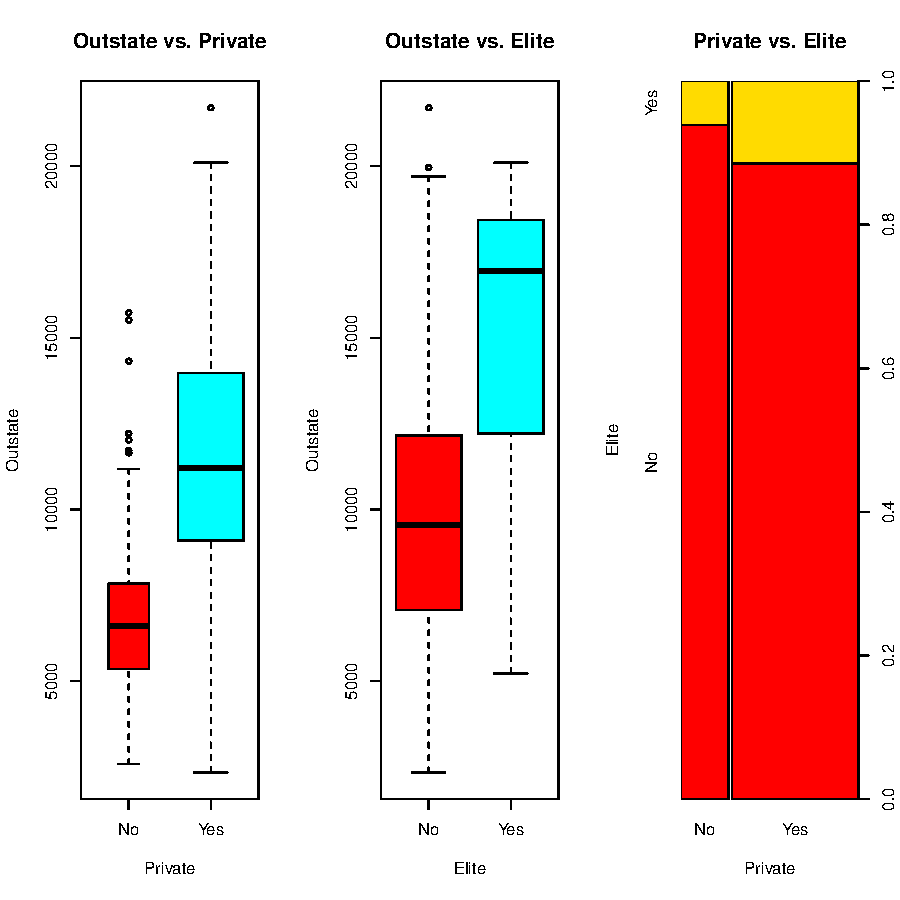
\includegraphics{introduction-outstate-private}

{
\colorbox{BurntOrange}{\textbf{discovery5:}}\color{red}\\
We can see that private school have far more outstate students, which means that private school are more attractive to outstate student.
}

\item Create a new qualitative variable, called Elite, by binning the Top10perc variable. We are going to divide universities into two groups based on whether or not the proportion of students coming from the top 10\% of their high school classes exceeds 50\%.

\begin{Schunk}
\begin{Sinput}
> Elite = rep("No", nrow(College))
> Elite[College$Top10perc > 50] = "Yes"
> Elite = as.factor(Elite)
> College = data.frame(College, Elite)
> summary(Elite)
\end{Sinput}
\begin{Soutput}
 No Yes 
699  78 
\end{Soutput}
\begin{Sinput}
> boxplot(Outstate ~ Elite, main = "Outstate vs. Elite", xlab = "Outstate", ylab = "Elite",
+         col = rainbow(2))
\end{Sinput}
\end{Schunk}
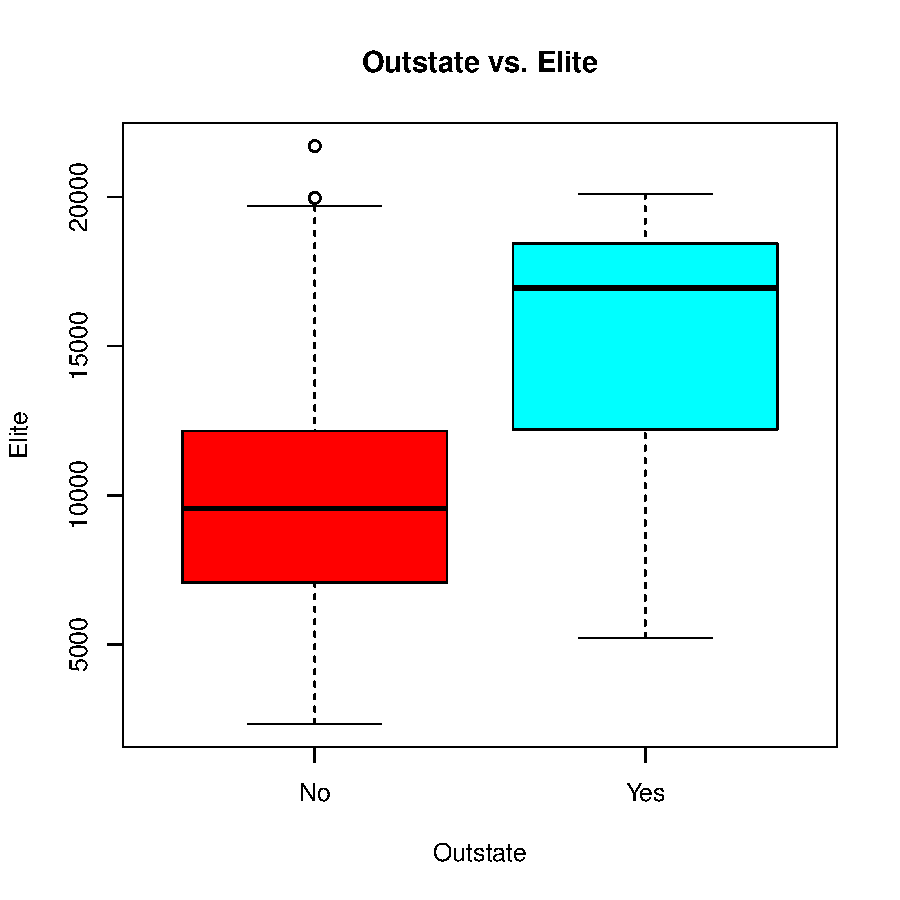
\includegraphics{introduction-outstate-elite}

{
\colorbox{BurntOrange}{\textbf{discovery6:}}\color{red}\\
From this picture we can see that the more outstate students, the more elite students. This makes us wander if the elite students are from outstate? Possible no. We need another expriment.
}


\item Plot Private vs. Elite
\begin{Schunk}
\begin{Sinput}
> plot(Private, Elite, main = "Private vs. Elite", xlab = "Private", ylab = "Elite",
+      col = rainbow(7))
\end{Sinput}
\end{Schunk}
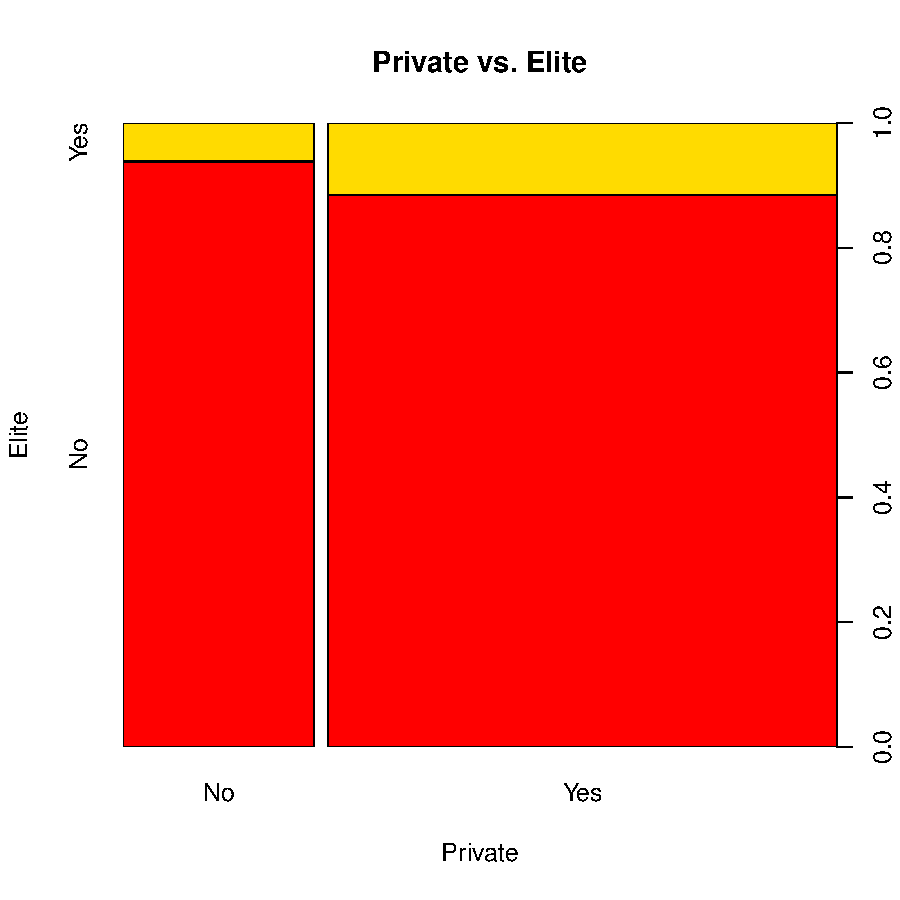
\includegraphics{introduction-Private-Elite}

{
\colorbox{BurntOrange}{\textbf{discovery7:}}\color{red}\\
Now it's clear that not only there are more private universities, but also there are more elite universities among private universities. So, it is because private schools are more attractive that they are more likely to be elite schools.
}


\item Use the hist() function to produce some histograms with differing numbers of bins for a few of the quantitative vari- ables.

\begin{Schunk}
\begin{Sinput}
> par(mfrow = c(3,3))
> hist(College$Apps, col = "red")
> hist(College$Top10perc, col = "blue")
> hist(College$Outstate, col = "green")
> hist(College$Room.Board, col = "yellow")
> hist(College$Personal, col = "pink")
> hist(College$S.F.Ratio, col = "brown")
> hist(College$PhD, col = "slateblue")
> hist(College$perc.alumni, col = "cadetblue1")
> hist(College$Grad.Rate, col = "sienna1")
\end{Sinput}
\end{Schunk}
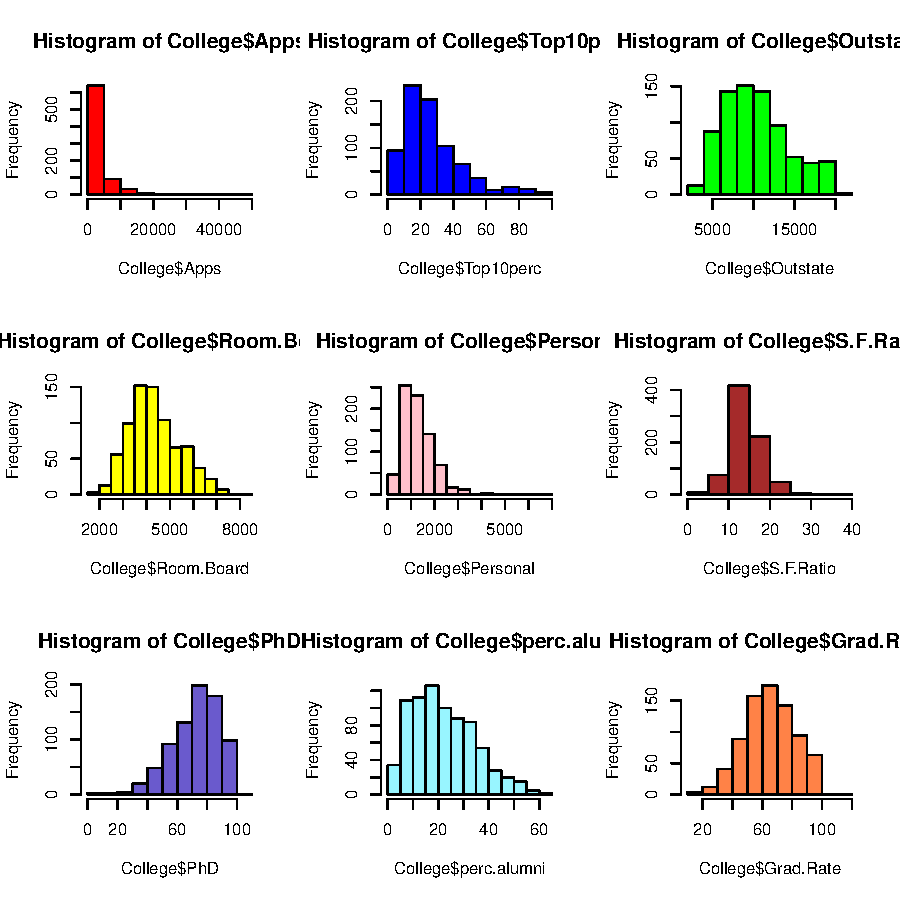
\includegraphics{introduction-hist}

{
\colorbox{BurntOrange}{\textbf{discovery8:}}\color{red}\\
Here we can see the distribution of the features of those 777 universities. It's easy to see that most schools have more than 70\% faculties that have PhD.; The expected probality that one graduate is 0.7, which is not bad, and so on.
}


\item Explore Northeastern:
\begin{Schunk}
\begin{Sinput}
> str(College[row.names(College) == "Northeastern University",])
\end{Sinput}
\begin{Soutput}
'data.frame':	1 obs. of  19 variables:
 $ Private    : Factor w/ 2 levels "No","Yes": 2
 $ Apps       : num 11901
 $ Accept     : num 8492
 $ Enroll     : num 2517
 $ Top10perc  : num 16
 $ Top25perc  : num 42
 $ F.Undergrad: num 11160
 $ P.Undergrad: num 10221
 $ Outstate   : num 13380
 $ Room.Board : num 7425
 $ Books      : num 600
 $ Personal   : num 1750
 $ PhD        : num 73
 $ Terminal   : num 82
 $ S.F.Ratio  : num 12.9
 $ perc.alumni: num 17
 $ Expend     : num 9563
 $ Grad.Rate  : num 46
 $ Elite      : Factor w/ 2 levels "No","Yes": 1
\end{Soutput}
\end{Schunk}

{
\colorbox{BurntOrange}{\textbf{discovery about Northeastern University:}}\color{red}\\
%\begin{comment}
I'm pretty interested in our schools features.
\begin{itemize}
\item We have more than 10000 applications, which really rare, which means our school is very attractive.
\item We accept more than 8000 students, more than 10000 full time and part time undergraduate student, which are all alse very uncommon. These figures makes me believe that our school is a very big school, which means that our school is really efficent at manage and organize student.
\item 16\% top10, 17\% donate alumni, 73\% PhD., 12.9\% S.F.Ratio, which are all normal level.
\item 7425 room \& board fees is twice the average level, makes our school expensive.
\item 46\% graduation is very low, which is absolutly not a good news for us.
\item our school is not a elite school
\end{itemize}
So, with the analysis above, Our school is a normal level, but very big, expensive school, with low probablity of gradutation.

%\end{comment}
}


\item Explore Elite Schools:
\begin{Schunk}
\begin{Sinput}
> sapply(College[College$Elite == "Yes", 2:18], mean)
\end{Sinput}
\begin{Soutput}
       Apps      Accept      Enroll   Top10perc   Top25perc F.Undergrad 
 5980.56410  2852.60256  1060.71795    67.61538    91.10256  4582.74359 
P.Undergrad    Outstate  Room.Board       Books    Personal         PhD 
  324.93590 15248.56410  5336.79487   594.91026  1188.17949    89.32051 
   Terminal   S.F.Ratio perc.alumni      Expend   Grad.Rate 
   94.08974    10.61410    33.96154 18404.87179    83.38462 
\end{Soutput}
\end{Schunk}

{
\colorbox{BurntOrange}{\textbf{discovery about Elite University:}}\color{red}\\
Here we can see a statistic summary about elite schools.\\
With comparision between NEU and those Elite schools, I provide that:
\begin{itemize}
\item Decrease acceptance, decrease enrollment.
\item Hire more PhD. teachers.
\item Find ways to ecourage our alumni to donate.
\item Find ways to increase graduatation percent.
\end{itemize}
}

\end{enumerate}


\newpage
\question{9}{Auto data set explore}

\begin{enumerate}
\item Load data, briefly looking what inside.
\begin{Schunk}
\begin{Sinput}
> library(ISLR)
> attach(Auto)
> str(Auto)
\end{Sinput}
\begin{Soutput}
'data.frame':	392 obs. of  9 variables:
 $ mpg         : num  18 15 18 16 17 15 14 14 14 15 ...
 $ cylinders   : num  8 8 8 8 8 8 8 8 8 8 ...
 $ displacement: num  307 350 318 304 302 429 454 440 455 390 ...
 $ horsepower  : num  130 165 150 150 140 198 220 215 225 190 ...
 $ weight      : num  3504 3693 3436 3433 3449 ...
 $ acceleration: num  12 11.5 11 12 10.5 10 9 8.5 10 8.5 ...
 $ year        : num  70 70 70 70 70 70 70 70 70 70 ...
 $ origin      : num  1 1 1 1 1 1 1 1 1 1 ...
 $ name        : Factor w/ 304 levels "amc ambassador brougham",..: 49 36 231 14 161 141 54 223 241 2 ...
\end{Soutput}
\begin{Sinput}
> summary(Auto)
\end{Sinput}
\begin{Soutput}
      mpg          cylinders      displacement     horsepower        weight    
 Min.   : 9.00   Min.   :3.000   Min.   : 68.0   Min.   : 46.0   Min.   :1613  
 1st Qu.:17.00   1st Qu.:4.000   1st Qu.:105.0   1st Qu.: 75.0   1st Qu.:2225  
 Median :22.75   Median :4.000   Median :151.0   Median : 93.5   Median :2804  
 Mean   :23.45   Mean   :5.472   Mean   :194.4   Mean   :104.5   Mean   :2978  
 3rd Qu.:29.00   3rd Qu.:8.000   3rd Qu.:275.8   3rd Qu.:126.0   3rd Qu.:3615  
 Max.   :46.60   Max.   :8.000   Max.   :455.0   Max.   :230.0   Max.   :5140  
                                                                               
  acceleration        year           origin                      name    
 Min.   : 8.00   Min.   :70.00   Min.   :1.000   amc matador       :  5  
 1st Qu.:13.78   1st Qu.:73.00   1st Qu.:1.000   ford pinto        :  5  
 Median :15.50   Median :76.00   Median :1.000   toyota corolla    :  5  
 Mean   :15.54   Mean   :75.98   Mean   :1.577   amc gremlin       :  4  
 3rd Qu.:17.02   3rd Qu.:79.00   3rd Qu.:2.000   amc hornet        :  4  
 Max.   :24.80   Max.   :82.00   Max.   :3.000   chevrolet chevette:  4  
                                                 (Other)           :365  
\end{Soutput}
\end{Schunk}

{
\colorbox{BurntOrange}{\textbf{discovery1:}}\color{red}\\
Here we find that Auto has 392 instances and each instance has 9 predictors\\
For all the predictors:
\begin{itemize}
\item quantitative predictors:
\begin{itemize}
\item mpg
\item displacement
\item horsepower
\item weight
\item acceleration
\end{itemize}

\item qualitative predictors:
\begin{itemize}
\item cylinders
\item year
\item origin
\item name
\end{itemize}

\end{itemize}
}

\item Make qualitative predictors as factors
\begin{Schunk}
\begin{Sinput}
> cylinders = as.factor(cylinders)
> year = as.factor(year)
> origin = as.factor(origin)
> name = as.factor(name)
\end{Sinput}
\end{Schunk}

\item Range of each quantitative predictor
\begin{Schunk}
\begin{Sinput}
> sapply(Auto[, c(1,3,4,5,6)], range)
\end{Sinput}
\begin{Soutput}
      mpg displacement horsepower weight acceleration
[1,]  9.0           68         46   1613          8.0
[2,] 46.6          455        230   5140         24.8
\end{Soutput}
\end{Schunk}


\item Mean and standard deviation of each quantitative predictor
\begin{Schunk}
\begin{Sinput}
> sapply(Auto[, c(1,3,4,5,6)], mean)
\end{Sinput}
\begin{Soutput}
         mpg displacement   horsepower       weight acceleration 
    23.44592    194.41199    104.46939   2977.58418     15.54133 
\end{Soutput}
\begin{Sinput}
> sapply(Auto[, c(1,3,4,5,6)], sd)
\end{Sinput}
\begin{Soutput}
         mpg displacement   horsepower       weight acceleration 
    7.805007   104.644004    38.491160   849.402560     2.758864 
\end{Soutput}
\end{Schunk}


\item Remove the 10th through 85th observations and recompute mean and std.
\begin{Schunk}
\begin{Sinput}
> n_row_names = as.numeric(rownames(Auto))
> selector = !(n_row_names >= 10 & n_row_names < 86)
> Auto2 = Auto[selector, ]
> sapply(Auto2[, c(1,3,4,5,6)], mean)
\end{Sinput}
\begin{Soutput}
         mpg displacement   horsepower       weight acceleration 
    24.36845    187.75394    100.95584   2939.64353     15.71830 
\end{Soutput}
\begin{Sinput}
> sapply(Auto2[, c(1,3,4,5,6)], sd)
\end{Sinput}
\begin{Soutput}
         mpg displacement   horsepower       weight acceleration 
    7.880898    99.939488    35.895567   812.649629     2.693813 
\end{Soutput}
\begin{Sinput}
> sapply(Auto2[, c(1,3,4,5,6)], range)
\end{Sinput}
\begin{Soutput}
      mpg displacement horsepower weight acceleration
[1,] 11.0           68         46   1649          8.5
[2,] 46.6          455        230   4997         24.8
\end{Soutput}
\end{Schunk}

{
\colorbox{BurntOrange}{\textbf{discovery2:}}\color{red}\\
After removing observations from 10th through 85th, we can see that range, mean and standard deviation do not change to much.
}


\item Graphical investigation of predictor
\begin{Schunk}
\begin{Sinput}
> pairs( ~mpg + displacement + horsepower + weight + acceleration , Auto)
\end{Sinput}
\end{Schunk}
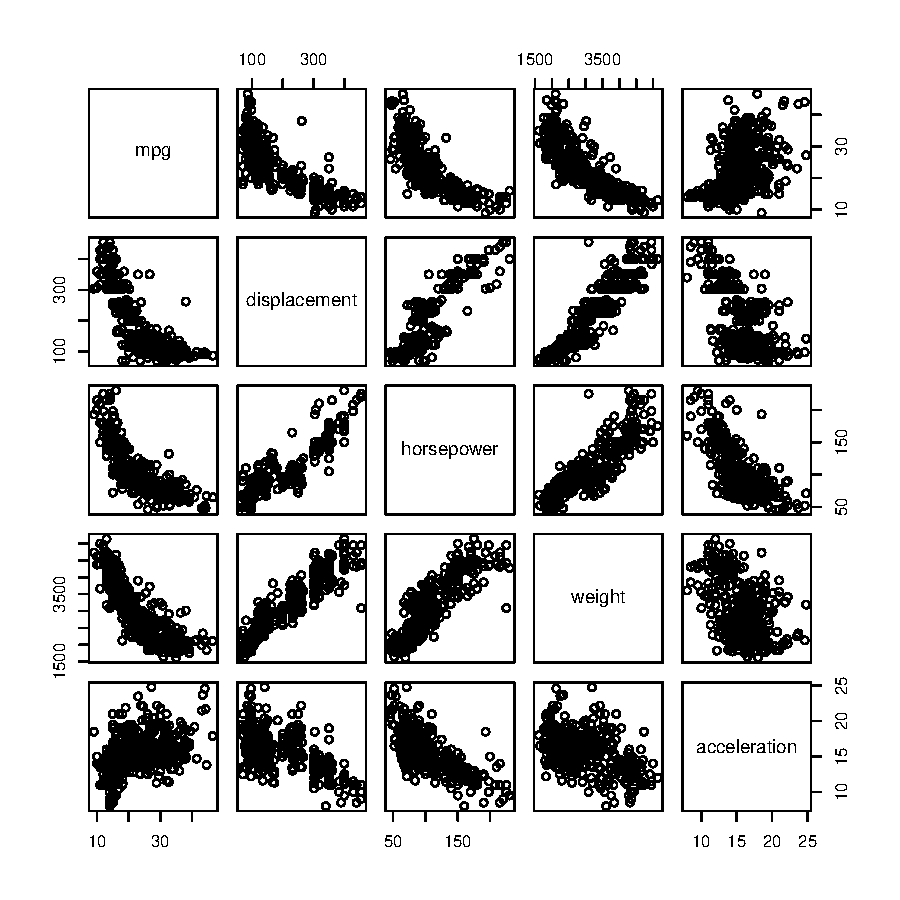
\includegraphics{introduction-pair}

\begin{Schunk}
\begin{Sinput}
> par(mfrow = c(3,3))
> boxplot(mpg ~ cylinders, col = rainbow(7), ylab = "mpg", xlab = "cylinders",
+         varwidth = T)
> plot(mpg ~ weight, col = rainbow(7))
> plot(mpg ~ horsepower, col = rainbow(7))
> boxplot(horsepower ~ cylinders, col = rainbow(7), ylab = "horsepower",
+         xlab = "cylinders", varwidth=T)
> boxplot(mpg ~ origin, col = rainbow(7), ylab = "mpg", xlab = "origin",
+         varwidth = T)
> boxplot(weight ~ origin, col = rainbow(7), ylab = "weight", xlab = "origin",
+         varwidth = T)
> boxplot(horsepower ~ origin, col = rainbow(7), ylab = "horsepower", xlab = "origin",
+         varwidth = T)
> boxplot(acceleration ~ origin, col = rainbow(7), ylab = "acceleration", xlab = "origin",
+         varwidth = T)
> boxplot(horsepower ~ year, col = rainbow(7), ylab = "horsepower", xlab = "year",
+         varwidth = T)
\end{Sinput}
\end{Schunk}
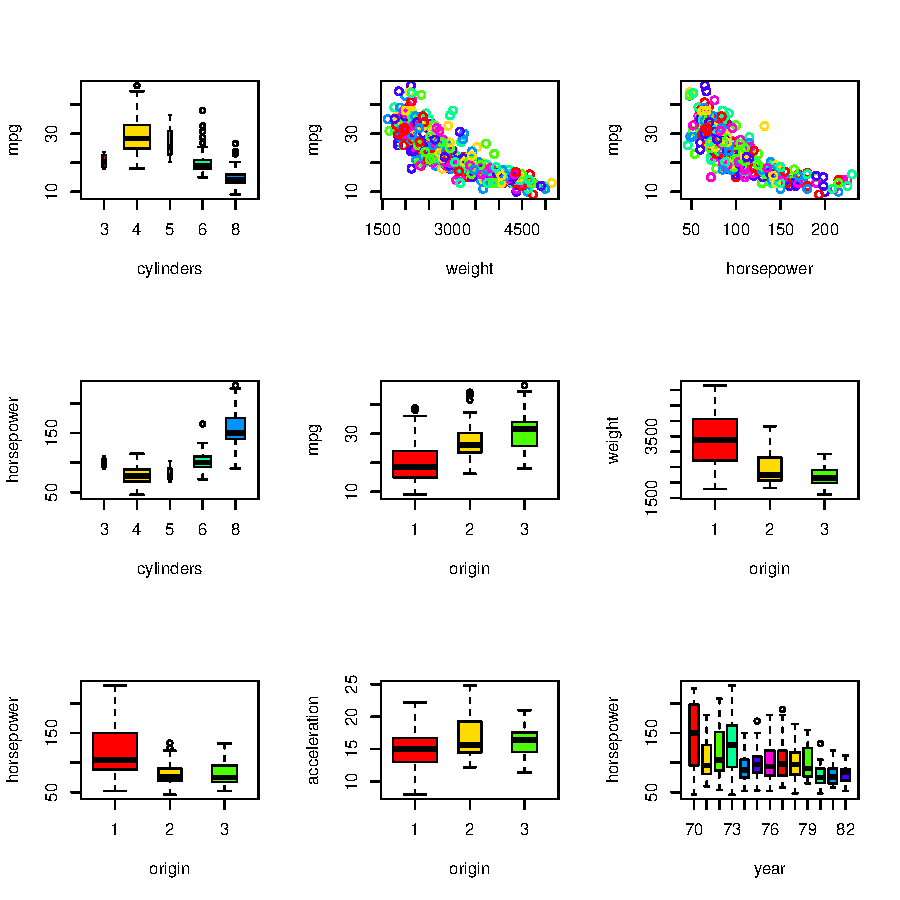
\includegraphics{introduction-mpg-cylinder}


{
\colorbox{BurntOrange}{\textbf{discovery3:}}\color{red}\\
Here we can get lots of information:
\begin{itemize}
\item Cars of 4 cylinders are most efficent with gas
\item The heavier the car, the more gas it consumes per mile
\item The more horsepower the car, the more gas it consumes per mile
\item The more cylinders one car have, the more horsepower. (which is common sense)
\item U.S. cars seem to consume more gas/mile than cars from other places
\item U.S. cars are tend to have more weith
\item U.S. cars have more horsepower
\item Europe cars accelerate faster
\item horsepower of cars decrease with years going on
\end{itemize}

It seems that if your are in U.S., buy yourself a nice car, which has more horsepower, heavier, even if it consumes more gas. But the good news is that the gas is pretty low compared with other countries(especially China).\\
\\
So, maybe it is because of low gas price that lead to the result that U.S. cars are generally more powerfull and heavier.\\
\\
My plots suggest that:\\
(1) The bigger the weight, the smaller the mpg\\
(2) 4 cylinders get the biggest mpg\\
(3) The bigger the horsepower, the smaller the mpg\\
Justify:\\
It's all about engine, heavier cars need more powerfull engine, which has more cylinders, more horsepower and consume more gas. In return, powerfull cars need to be built with more weight to keep it stable in high speed.
}

\end{enumerate}

\end{document}
